\documentclass{beamer}
\usepackage[utf8]{inputenc}

%\usetheme{Madrid}
\setbeameroption{show notes}
\beamertemplatenavigationsymbolsempty
\hypersetup{hidelinks}

\usepackage{listings}
\lstset{language=[ISO]C++,
        basicstyle=\ttfamily\scriptsize,
        keywordstyle=\color{blue},
        stringstyle=\color{red},
        commentstyle=\color{green},
        frame=single,
        showspaces=false,
        }

\lstdefinelanguage{cmake}
{
  morekeywords=
  {
    add_executable, target_link_libraries, add_test,
  },
}

\usepackage{lmodern}
\usepackage{color}
\usepackage[backend=biber]{biblatex}
\bibliography{script}

\title{Advanced programming}
\author{David Schneider}
\date{2016}

\AtBeginPart{\frame{\partpage}\frame{\frametitle{Content Part
\insertpart}\tableofcontents}}

\begin{document}

\frame{\titlepage}

\part{Overview}

\section{Über mich}

\begin{frame}{Über mich}
\begin{block}{Name}
David Schneider
\end{block}

\begin{block}{Kontakt}
E-Mail: \\
\url{schneidav81@gmail.com} \\
\url{david.schneider@fhwn.ac.at} \\
Telefon: 0680 1454649
\end{block}

\end{frame}

\begin{frame}{Erfahrungen}

\begin{block}{Ausbildung}
\begin{itemize}
  \item Elektroniker Lehre mit Berufsmatura
  \item Zürcher Fachhochschule, Elektrotechnik, Vertiefung Regelungstechnik und
Computertechnik
\end{itemize}
\end{block}

\begin{block}{Berufserfahrung}
\begin{itemize}
  \item Messsystem für hochprezise Temperaturmessung, IST AG
  \item Message Gateway für SMS, Dimoco
  \item Automotiv Steuergeräte für Scheinwerfer, ZKW
\end{itemize}
\end{block}

\end{frame}

\section{Overview}

%%%%%%%%%%%%%%%%%%%%%%%%%%%%%%%%%%%%%%%%%%%%%%%%%%%%%%%%%%%%%%%%%%%%%
\begin{frame}{Modalitäten}
\begin{description}
\item[Umfang] 5 ECTS
\item[Lehr- und Lernformen]: Vorlesung mit integrierter Übung
\item[Prüfungsmodalitäten]: LV-abschließende Prüfung; Projektarbeit - Prüfungsgespräch über die Projektarbeit
\end{description}
\end{frame}

%%%%%%%%%%%%%%%%%%%%%%%%%%%%%%%%%%%%%%%%%%%%%%%%%%%%%%%%%%%%%%%%%%%%%
\begin{frame}{Lehrinhalte}
Erlernen von Konzepten der objektorientierten Programmierung anhand der
Programmiersprache C++ (Klassen und Objekte, Kapselung, Vererbung und
Polymorphismus), Fehler- und Ausnahmebehandlung, Coding Guidelines, Design
Patterns, Design for Testability. Bildung von Modellen, Abstraktion,
Lösungsfindung und Evaluation in der  objektorientierten Programmierung.
Einbindung vorhandener Lösungskonzepte und systematische Herangehensweise an
konkreten Problemstellungen.
\end{frame}

%%%%%%%%%%%%%%%%%%%%%%%%%%%%%%%%%%%%%%%%%%%%%%%%%%%%%%%%%%%%%%%%%%%%%
\begin{frame}{Literaturempfehlungen}
\begin{itemize}
\item E. Gamma et al., Design Patterns, Addison-Wesley (1995)
\item R. Martin, Clean Code, Prentice Hall Pearson Education (2009)
\item B. Stroustrup: The C++ Programming Language, 4th edition, Addison Wesley
(2013)
\item A. Alexandrescu: Modern C++ Design, Addison Wesley (2001)
\item H. Sutter: C++ Coding Standards, Addison Wesley (2004)
\end{itemize}
\end{frame}

\begin{frame}{Termine 2016}
\begin{table}
\begin{tabular}{l | l }
Datum & Raum \\
\hline
23. September 2016 & EDV5 \\
30. September 2016 & EDV2 \\
07. Oktober 2016 & EDV2 \\
14. Oktober 2016 & EDV2 \\
21. Oktober 2016 & EDV2 \\
28. Oktober 2016 & EDV2 \\
04. November 2016 & EDV2 \\
11. November 2016 & EDV2 \\
18. November 2016 & EDV2 \\
25. November 2016 & EDV2
\end{tabular}
\end{table}
\end{frame}

\begin{frame}{Themen}
\begin{itemize}
  \item Objekt-Orientieres Design
  \item Einführung in C++
  \item Clean Code
  \item Unit Testing
  \item Software Development Methodology
  \item Coding Standards
\end{itemize}
\end{frame}

\section{Einstufung}
\begin{frame}[fragile]{Frage 1}
Was ist der output von folgendem Code:
\begin{lstlisting}
for (int i = 0; i < 5; ++i)
{
  std::cout << i << std::endl;
}
\end{lstlisting}
\end{frame}

\begin{frame}{Frage 2}
Was ist der Unterschied zwischen Stack und Heap? Wann wir welcher Speicher
verwended? Wie wird eine Stack-Variable deklariert und wie eine Heap-Variable?
\end{frame}

\begin{frame}[fragile]{Frage 3}
Was ist der Typ und der Wert des folgenden Ausdrucks?
\begin{lstlisting}
int x = 12;
int y = 7;

(x != 4) || (y == 2)
\end{lstlisting}
\end{frame}

\begin{frame}[fragile]{Frage 4}
Was ist der Inhalt der Variablen str und p?
\begin{lstlisting}
char str[20] = "Hello";
char *const p = str;
*p = 'M';
\end{lstlisting}
\end{frame}

\part{Introduction}

\section{Introduction}

\subsection{Object-oriented programming}

\begin{frame}{Pradigma}
OOP is a programming paradigm
\begin{block}{Objects contain}
\begin{itemize}
\item data (ak. attribute)
\item code (ak. methods)
\end{itemize}
\end{block}
\end{frame}

\begin{frame}{OOP vs. Procedural}

\begin{block}{Procedural}
data tends to be highly decoupled from the functions that operate on it
\end{block}

\begin{block}{Object-oriented}
data tends to carry with it a collection of functions
\end{block}

\footfullcite{Stackoverflow1}

\end{frame}

\subsection{Object-oriented concepts}

\begin{frame}{Classes and objects}

\begin{block}{Class}
The blueprint for an object. Defines how a object should be created.
\end{block}

\begin{block}{Object}
An instance of a class. Gets created during runtime.
\end{block}

\end{frame}

\begin{frame}{Information hidding}
Encapsulate data and hide the internal structure from caller. This allows
changing the internal details without affecting.
\end{frame}

\begin{frame}{Inheritance}
Inheritance is when a class is based on another class, using the same
implementation to maintain the same behavior.
Such an inherited class is called a subclass of its parent class or super class.
It is a mechanism for code reuse and to allow independent extensions of the
original software via public classes and interfaces.
 Often called a `Is-A-Relation`.
\end{frame}

\begin{frame}{Interface}
Define a method without implementing it as an interface to be used by other
classes. \\
A interface is often called `an abstract base class`.
\end{frame}

\begin{frame}{Polymorphism}
\framesubtitle{aka Subtyping}
Polymorphism is the provision of a single interface to entities of different
types.

Define a implementation for a specialized type. Or change the behavior of a
class by subtyping it and overwrite a method.
\end{frame}

\subsection{C++}
\begin{frame}{C++ - Overview}
\begin{itemize}
  \item compiled language
  \item general-purpose programming language
  \item Multi-pradigma
  \begin{itemize}
    \item procedural
    \item functional
    \item object-oriented
    \item generic
  \end{itemize}
  \item statically typed
  \item allows low-level memory manipulation
  \item designed for large, resource constrained systems 
\end{itemize}
\end{frame}


\begin{frame}{C++ - Standardization}
\itemize{}
\item[1979] C with Classes first implemented 
\item[1998] C++98 (ISO/IEC 14882:1998)
\item[2003] C++03 (ISO/IEC 14882:2003)
\item[2011] C++11 (ISO/IEC 14882:2011)
\item[2014] C++14 (ISO/IEC 14882:2014)
\item[2017] C++17 (also called C++1z)
\end{frame}

\begin{frame}{The Boost Library}
\begin{itemize}
  \item Started arround 1999
  \item several Boost libraries have been accepted for incorporation into the
  C++11 standard.
\end{itemize}
\end{frame}

\begin{frame}{Emedded Systems}
\begin{itemize}
  \item Embedded C++ (still in use?)
\end{itemize}
\end{frame}


\part{Buildsystem}

\section{Buildsystem}
\subsection{Tools}
\begin{frame}{Tools}
\begin{description}
  \item[Code:Blocks] \url{http://www.codeblocks.org/}
  \item[Git for Windows] \url{https://git-for-windows.github.io/}
  \item[TortoiseGit] \url{https://tortoisegit.org/}
  \item[CMake] \url{https://cmake.org/}  
\end{description}

\end{frame}

\part{OO-Basics}

\section{OO-Basics}

\begin{frame}
Design is all about changable code.
Code is written once, but read many times.
\end{frame}

\subsection{Features}

\begin{frame}
accessibility
\end{frame}

\begin{frame}{Encapsulation}
abstraction
information hidding
hide internal details, which allows changing this details
\end{frame}

\begin{frame}{Inheritance}
Base class
Abstract class
\end{frame}

\begin{frame}{Composition and delegation}
% TODO Composition and delegation
\end{frame}

\begin{frame}{Polymorphism}
subtyping
\end{frame}

\begin{frame}{Open recursion}
Virtual methods

\lstinputlisting[caption=Open recursion]{lst/open_recursion.cpp}


\end{frame}


\section{SOLID}

\begin{frame}{S.O.L.I.D - Principals}
Defined by Robert C. Martin (Oncle Bob)

\begin{description}
\item [S] Single-responsiblity principle
\item [O] Open-closed principle
\item [L] Liskov substitution principle
\item [I] Interface segregation principle
\item [D] Dependency Inversion Principle
\end{description}
\end{frame}

\subsection{Single-responsiblity principle}

\begin{frame}[fragile]{Single-responsiblity principle}
''A class should have only a single responsibility.''
\end{frame}

\begin{frame}[fragile]{SRP - Example}
\begin{lstlisting}[caption=SRP Anti-Example]
class Report
{
  void collectData();
  void print();
};
\end{lstlisting}

\begin{block}{Reasons to change:}
\begin{itemize}
  \item The content of the report could change.
  \item The report format chould change.
\end{itemize}
\end{block}
\end{frame}


\subsection{Open-closed principle}

\begin{frame}{Open-closed principle}
''Software entities (classes, modules, functions, etc.) should be open for
extension, but closed for modification.'
\end{frame}

\begin{frame}[fragile]{OCP - Example}
Adding an new class should lead to no or very little changes at the existing
code.

\begin{lstlisting}[caption=OCP Anti-Example]
class Square {
  float length;
};

class Circle {
  float radius;
};

class AreaCalculator {
  float area(const Square& square) {
    return std::pow(square.length);
  }
  
  float area(const Circle& circle) {
    return std::pow(circle.radius) * M_PI;
  }
};
\end{lstlisting}
\end{frame}

\begin{frame}[fragile]{OCP - Example}
\begin{lstlisting}[caption=OCP Example]
class Shape {
  virtual float area() = 0;
};

class Square : public Shape {
  float length;
  float area() {
    return std::pow(this->length);
  }
};

class Circle : public Shape {
  float radius;
  float area() {
    return std::pow(this->radius) * M_PI;
  }
};

class AreaCalculator {
  float area(const Shape& shape) {
    return shape.area();
  }
};
\end{lstlisting}
\end{frame}


\subsection{Liskov substitution principle}

\begin{frame}{Liskov substitution principle}
''Subtypes must be substitutable for their base types.''
\end{frame}

\begin{frame}[fragile]{LSP - Example}
\begin{lstlisting}[caption=LSP Example]
class Vehicle {
  virtual void startEngine() {
    // Default engine start functionality
  }
};

class Car : public Vehicle {
  void startEngine() {
    this->engageIgnition();
    Vehicle::startEngine();
  }

  void engageIgnition() {
    // Ignition procedure
  }
};
\end{lstlisting}
Example of LSP Violation: `Square is-a Rectangle`
\end{frame}


\subsection{Interface segregation principle}

\begin{frame}{Interface segregation principle}
''Many client specific interfaces are better than one general purpose
interface''
\end{frame}

\begin{frame}{ISP - Example}
% TODO ISP Example
\end{frame}


\subsection{Dependency Inversion Principle}

\begin{frame}{Dependency Inversion Principle}
\end{frame}

\section{Programming idiom}
\frame{RAII - Resource Acquisition Is Initialization}

\frame{PImpl - Pointer To Implementation}

\section{Clean Code}
\begin{frame}{Clean Code}
% TODO Clean Code
\end{frame}

\part{Object Oriented Design - Pattern}
\section{Object Oriented Design - Pattern}

\begin{frame}{Pattern}
\begin{itemize}
  \item singelton
  \item factory
  \item command
  \item observer
  \item strategy
  \item visitor
  \item null object
  \item adapter
  \item proxy
  \item fly-weight
\end{itemize}
\end{frame}

\part{C++ Tutorial}{cpp-tutorial}

\begin{frame}{Source}
C++ Language Tutorial
Source: \url{http://www.cplusplus.com/doc/tutorial/}
\begin{block}

reference on cplusplus.com contains some errors,
\url{http://stackoverflow.com/questions/6520052/whats-wrong-with-cplusplus-com}
\end{block}
\end{frame}

\section{Basics of C++}

\subsection{Structure of a program}
\begin{frame}{Structure of a program}
% TODO Structure of a program
\end{frame}

\subsection{Variables and types}
\begin{frame}{Variables and types}
% TODO Variables and types
\end{frame}


%%%%%%%%%%%%%%%%%%%%%%%%%%%%%%%%%%%%%%%%%%%%%%%%%%%%%%%%%%%%%%%%%%%%%
\begin{frame}[fragile]{Identifiers}
\begin{itemize}
  \item case-sensitive
  \item sequence of one or more letters, digits, or underscore
  \item always begin with a letter
  \item begin with underscore allowd, but used for special cases
  \item many reserved keywords, which can't be used as identifiers 
\end{itemize}
\begin{lstlisting}[caption=Identifiers Examples]
aNumber
my1st_variable
SomeMoreIdentifier
\end{lstlisting}
\end{frame}

%%%%%%%%%%%%%%%%%%%%%%%%%%%%%%%%%%%%%%%%%%%%%%%%%%%%%%%%%%%%%%%%%%%%%
\begin{frame}{Fundamental data types}
\begin{itemize}
  \item Character types
  \item Numerical integer types
  \item Floating-point types
  \item Boolean type
\end{itemize}
\end{frame}

%%%%%%%%%%%%%%%%%%%%%%%%%%%%%%%%%%%%%%%%%%%%%%%%%%%%%%%%%%%%%%%%%%%%%
\begin{frame}{Fundamental data types}
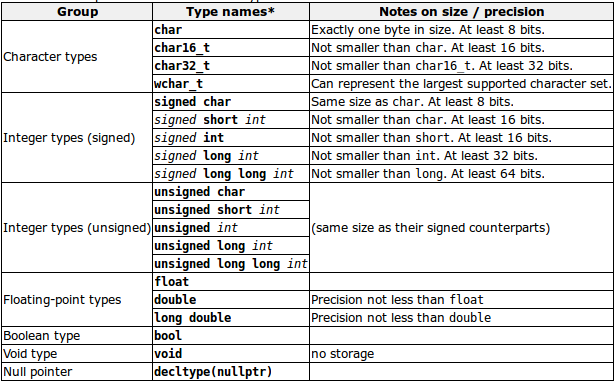
\includegraphics[scale=0.48]{img/FundamentalTypes.png}
\end{frame}

%%%%%%%%%%%%%%%%%%%%%%%%%%%%%%%%%%%%%%%%%%%%%%%%%%%%%%%%%%%%%%%%%%%%%
\begin{frame}[fragile]{Declaration of variables}
\begin{itemize}
  \item Strongly typed
  \item Every variable to be declared before first use
\end{itemize}
\begin{lstlisting}[caption=Variable declaration]
int aNumber;
float aFloatingPointerNumber;
\end{lstlisting}
\end{frame}

%%%%%%%%%%%%%%%%%%%%%%%%%%%%%%%%%%%%%%%%%%%%%%%%%%%%%%%%%%%%%%%%%%%%%
\begin{frame}[fragile]{Initialization of variables}
\begin{definition}{Initialization}
   Set the value of variable during declaration. 
\end{definition}
\begin{lstlisting}[caption=Variable initialization]
int aNumber = 5;
float aFloatingPointerNumber(6);
\end{lstlisting}
\end{frame}

%%%%%%%%%%%%%%%%%%%%%%%%%%%%%%%%%%%%%%%%%%%%%%%%%%%%%%%%%%%%%%%%%%%%%
\begin{frame}[fragile]{Type deduction: auto and decltype}
Automatic type determination with keyword `auto`.

Usefull for cases where the explicitly type is not so importent or the type is
so complex (ex. with templates) that it's hard the define the type correct.

\lstinputlisting[caption=Auto Type]{lst/AutoType.cpp}

\end{frame}

%%%%%%%%%%%%%%%%%%%%%%%%%%%%%%%%%%%%%%%%%%%%%%%%%%%%%%%%%%%%%%%%%%%%%
\begin{frame}{Introduction to strings}
Example for compound types: std::string

\lstinputlisting[caption=String Example]{lst/SimpleString.cpp}

\end{frame}


\subsection{Constants}

%%%%%%%%%%%%%%%%%%%%%%%%%%%%%%%%%%%%%%%%%%%%%%%%%%%%%%%%%%%%%%%%%%%%%
\begin{frame}[fragile]{Literals}

\begin{lstlisting}[caption=Integer Numerals]
75         // decimal
0113       // octal
0x4b       // hexadecimal
\end{lstlisting}

\end{frame}

%%%%%%%%%%%%%%%%%%%%%%%%%%%%%%%%%%%%%%%%%%%%%%%%%%%%%%%%%%%%%%%%%%%%%
\begin{frame}[fragile]{Literals}

\begin{lstlisting}[caption=Floating Point Numerals]
3.14159    // 3.14159
6.02e23    // 6.02 x 10^23
1.6e-19    // 1.6 x 10^-19
3.0        // 3.0
\end{lstlisting}

\end{frame}

%%%%%%%%%%%%%%%%%%%%%%%%%%%%%%%%%%%%%%%%%%%%%%%%%%%%%%%%%%%%%%%%%%%%%
\begin{frame}{Literals}
\begin{table}
\begin{tabular}{l | c}
Suffix & Type modifier \\
\hline
u or U & unsigned \\
l or L & long \\
ll or LL & long long \\
f or F & float \\
l or L & long double
\end{tabular}
\caption{Type modifier}
\end{table}

\end{frame}

%%%%%%%%%%%%%%%%%%%%%%%%%%%%%%%%%%%%%%%%%%%%%%%%%%%%%%%%%%%%%%%%%%%%%
\begin{frame}[fragile]{Character and string literals}
\begin{description}
\item[Character] A singel character, between single quotes
\item[String] Null-terminated string, between double quotes 
\end{description}
\begin{lstlisting}[caption=Character and string literals]
'z'
'p'
"Hello world"
"How do you do?"
\end{lstlisting}

\end{frame}

%%%%%%%%%%%%%%%%%%%%%%%%%%%%%%%%%%%%%%%%%%%%%%%%%%%%%%%%%%%%%%%%%%%%%
\begin{frame}[fragile]{Other literals}
\begin{description}
\item[Boolean] true and false
\item[Null-Pointer] reserved value to indicated, that a pointer doesn't refer to
a valid object
\end{description}
\begin{lstlisting}[caption=Other literals]
bool foo = true;
bool bar = false;
int* p = nullptr;
\end{lstlisting}
\end{frame}

%%%%%%%%%%%%%%%%%%%%%%%%%%%%%%%%%%%%%%%%%%%%%%%%%%%%%%%%%%%%%%%%%%%%%
\begin{frame}[fragile]{Typed constant expressions}
\begin{lstlisting}[caption=Typed constant expressions]
const double pi = 3.1415926;
const char tab = '\t';
\end{lstlisting}
\end{frame}

%%%%%%%%%%%%%%%%%%%%%%%%%%%%%%%%%%%%%%%%%%%%%%%%%%%%%%%%%%%%%%%%%%%%%
\begin{frame}[fragile]{Preprocessor definitions}
\begin{lstlisting}[caption=Preprocessor definitions]
#define PI 3.14159
#define NEWLINE '\n'
\end{lstlisting}
\end{frame}


\subsection{Operators}

\begin{frame}[fragile]{Assignment operator}
\begin{definition}
The assignment operator assigns a value to a variable.
\end{definition}

\begin{lstlisting}[caption=Assignment operator]
a = 5;
\end{lstlisting}

\end{frame}

%%%%%%%%%%%%%%%%%%%%%%%%%%%%%%%%%%%%%%%%%%%%%%%%%%%%%%%%%%%%%%%%%%%%%
\begin{frame}[fragile]{Arithmetic operators}
\begin{table}
\begin{tabular}{l | l}
operator & description \\
\hline
+ & addition \\
- & subtraction \\
* & multiplication \\
/ & division \\
\% & modulo
\end{tabular}
\caption{Arithmetic operators}
\end{table}
\begin{lstlisting}[caption=Modulo operator]
a = 11 % 3;
\end{lstlisting}
\end{frame}

%%%%%%%%%%%%%%%%%%%%%%%%%%%%%%%%%%%%%%%%%%%%%%%%%%%%%%%%%%%%%%%%%%%%%
\begin{frame}[fragile]{Compound assignment}
\begin{table}
\begin{tabular}{l | l}
expression & equivalent to... \\
\hline
y += x; & y = y + x; \\
x -= 5; & x = x - 5; \\
x /= y; & x = x / y; \\
price *= units + 1; & price = price * (units+1);
\end{tabular}
\caption{Compound assignment}
\end{table}
\begin{lstlisting}[caption=Modulo operator]
a += 2;   // equivalent to a=a+2
\end{lstlisting}
\end{frame}

%%%%%%%%%%%%%%%%%%%%%%%%%%%%%%%%%%%%%%%%%%%%%%%%%%%%%%%%%%%%%%%%%%%%%
\begin{frame}{Increment and decrement}
\begin{table}
\begin{tabular}{l | l}
operator & description \\
\hline
++ & increase operator \\
-- & decrease operator
\end{tabular}
\end{table}

%%%%%%%%%%%%%%%%%%%%%%%%%%%%%%%%%%%%%%%%%%%%%%%%%%%%%%%%%%%%%%%%%%%%%
\begin{table}
\begin{tabular}{l | l}
prefix & modifies the variable after evaluating \\
postfix & modifies the variable before evaluating
\end{tabular}
\end{table}
\end{frame}

%%%%%%%%%%%%%%%%%%%%%%%%%%%%%%%%%%%%%%%%%%%%%%%%%%%%%%%%%%%%%%%%%%%%%
\begin{frame}{Relational and comparison operators}
\begin{table}
\begin{tabular}{l | l}
operator & description \\
\hline
== & Equal to \\
!= & Not equal to \\
< & Less than \\
> & Greater than \\
<= & Less than or equal to \\
>= & Greater than or equal to
\end{tabular}
\caption{Relational and comparison operators}
\end{table}
\end{frame}

%%%%%%%%%%%%%%%%%%%%%%%%%%%%%%%%%%%%%%%%%%%%%%%%%%%%%%%%%%%%%%%%%%%%%
\begin{frame}{Logical operators}
\begin{table}
\begin{tabular}{l | l}
operator & description \\
\hline
\&\& & logical-and \\
\textbar\textbar & logical-or \\
! & logical-not
\end{tabular}
\caption{Logical operators}
\end{table}
\end{frame}

%%%%%%%%%%%%%%%%%%%%%%%%%%%%%%%%%%%%%%%%%%%%%%%%%%%%%%%%%%%%%%%%%%%%%
\begin{frame}{Bitwise operators}
\begin{table}
\begin{tabular}{l | l}
operator & description \\
\hline
\& & Bitwise AND \\
\textbar & Bitwise inclusive OR \\
\textasciitilde & Unary complement (bit inversion) \\
<< & Shift bits left \\
>> & Shift bits right
\end{tabular}
\caption{Bitwise operators}
\end{table}
\end{frame}

%%%%%%%%%%%%%%%%%%%%%%%%%%%%%%%%%%%%%%%%%%%%%%%%%%%%%%%%%%%%%%%%%%%%%
\begin{frame}[fragile]{Explicit type casting operator}
\begin{lstlisting}[caption=Type cast]
uint16_t a;
uint16_t b;

uint32_t sum = (uint32_t)a + b;
\end{lstlisting}
\end{frame}

%%%%%%%%%%%%%%%%%%%%%%%%%%%%%%%%%%%%%%%%%%%%%%%%%%%%%%%%%%%%%%%%%%%%%
\begin{frame}{Precedence of operators}
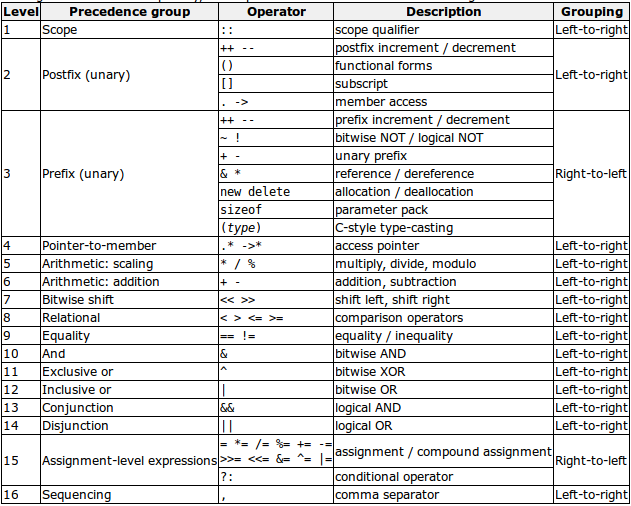
\includegraphics[scale=0.48]{img/OperatorPrecedence.png}
\end{frame}


\subsection{Basic Input/Output}

%%%%%%%%%%%%%%%%%%%%%%%%%%%%%%%%%%%%%%%%%%%%%%%%%%%%%%%%%%%%%%%%%%%%%
\begin{frame}{Streams}
\begin{itemize}
\item Abstraction `Streams` for input and output operations
\item Media independed (examples: file, consol, socket)
\item streams are a source/destination of characters
\item characters are provided/accepted sequentially
\end{itemize}
\end{frame}

%%%%%%%%%%%%%%%%%%%%%%%%%%%%%%%%%%%%%%%%%%%%%%%%%%%%%%%%%%%%%%%%%%%%%
\begin{frame}{Standard libray streams}
\begin{table}
\begin{tabular}{l | l}
stream & description \\
\hline
cin & standard input stream \\
cout & standard output stream \\
cerr & standard error (output) stream \\
clog & standard logging (output) stream \\
\end{tabular}
\caption{Bitwise operators}
\end{table}
\end{frame}

%%%%%%%%%%%%%%%%%%%%%%%%%%%%%%%%%%%%%%%%%%%%%%%%%%%%%%%%%%%%%%%%%%%%%
\begin{frame}[fragile]{Standard output (cout)}
\begin{lstlisting}[caption=Standard output]
// prints Output sentence on screen
std::cout << "Output sentence" 

// prints number 120 on screen
std::cout << 120;

// prints the value of x on screen
std::cout << x;
\end{lstlisting}
\end{frame}

%%%%%%%%%%%%%%%%%%%%%%%%%%%%%%%%%%%%%%%%%%%%%%%%%%%%%%%%%%%%%%%%%%%%%
\begin{frame}[fragile]{New line}
\begin{lstlisting}[caption=Use ASCII newline character]
std::cout << "First sentence.\n";
std::cout << "Second sentence.\nThird sentence.";
\end{lstlisting}

\begin{lstlisting}[caption=Use portable endl]
std::cout << "First sentence." << std::endl;
std::cout << "Second sentence." << std::endl
          << "Third sentence.";
\end{lstlisting}
\end{frame}

%%%%%%%%%%%%%%%%%%%%%%%%%%%%%%%%%%%%%%%%%%%%%%%%%%%%%%%%%%%%%%%%%%%%%
\begin{frame}[fragile]{Standard input (cin)}
\begin{itemize}
\item Input is only processed after `ENTER` key pressed
\item If conversion fails, not value is assigned
\item Spaces are always consideres as value terminator, which makes it difficult
to read a whole sentense into a string
\end{itemize}

\begin{lstlisting}[caption=Standard input]
int i;
std::cout << "Please enter an integer value: ";
std::cin >> i;
std::cout << "The value you entered is " << i;
std::cout << " and its double is " << i*2 << "." 
          << std::endl;
\end{lstlisting}
\end{frame}


\section{Program structure}

%%%%%%%%%%%%%%%%%%%%%%%%%%%%%%%%%%%%%%%%%%%%%%%%%%%%%%%%%%%%%%%%%%%%%
\begin{frame}[fragile]{Single statment vs. compound statement}
Where ever a single statement can be used, also a compound statement (block) can
be inserted.  compound statement is a group of statements (each of them
terminated by its own semicolon), but all grouped together in a block, enclosed 
in curly braces: {}:
\begin{lstlisting}[caption=Compound statement]
{ 
  statement1; 
  statement2; 
  statement3;
}
\end{lstlisting}
\end{frame}


\subsection{Statements and flow control}
%%%%%%%%%%%%%%%%%%%%%%%%%%%%%%%%%%%%%%%%%%%%%%%%%%%%%%%%%%%%%%%%%%%%%
\begin{frame}[fragile]{Selection statements}
\begin{lstlisting}[caption=If and else]
if (expression)
  statement;
else
  statement;
\end{lstlisting}

\begin{lstlisting}[caption=Switch]
switch (expression)
{
  case constant1:
     statement;
     break;
  case constant2:
     statement;
     break;
  default:
     statement;
}
\end{lstlisting}

\end{frame}

\begin{frame}{Iteration statements (loops)}
\begin{itemize}
  \item while (expression) statement;
  \item do statement while (condition);
  \item for (initialization; condition; increase) statement;
  \item for ( declaration : range ) statement;
\end{itemize}
\end{frame}

\begin{frame}{Jump statements}
\begin{itemize}
  \item The break statement
  \item The continue statement
  \item The goto statement
\end{itemize}
\end{frame}

\subsection{Functions}
\begin{frame}
\lstinputlisting[caption=Function example]{lst/Function.cpp}
\end{frame}

\begin{frame}[fragile]{Arguments passed by value and by reference}
\begin{description}
\item[pass by value] Value is copied
\item[pass by reference] Value is referenced
\end{description}
\begin{lstlisting}[caption=Const reference parameter]
std::string concatenate(const std::string& a,
                        const std::string& b)
{
  return a + b;
}
\end{lstlisting}
\end{frame}

\begin{frame}[fragile]{Default values in parameters}
\lstinputlisting[caption=Default value example]{lst/DefaultValue.cpp}
\end{frame}

\subsection{Overloads and templates}
\begin{frame}[fragile]{Overloaded functions}
\begin{lstlisting}[caption=Overloaded functions]
int operate(int a, int b)
{
  return a * b;
}

double operate(double a, double b)
{
  return a / b;
}
\end{lstlisting}
\end{frame}

\begin{frame}[fragile]{Templates}
\begin{lstlisting}[caption=Templates]
template <class T>
T sum(T a, T b)
{
  return a + b;
}\end{lstlisting}
\end{frame}

\subsection{Name visibility}
\begin{frame}{Scopes}
\begin{description}
\item[global scope] valid anywhere in the code
\item[namespace scope] group of entities in global scope
\item[local scope] only visible within the specific block in which it is
declared
\end{description}
\end{frame}

\begin{frame}[fragile]{Namespaces}
\begin{lstlisting}[caption=Namespace]
namespace myNamespace
{
  int a;
  float b;
}

void foo()
{
  std::cout << myNamespace::a;
}
\end{lstlisting}
\end{frame}

\begin{frame}[fragile]{Using}
The keyword using introduces a name into the current declarative region (such as
a block), thus avoiding the need to qualify the name.
\begin{lstlisting}[caption=using]
void foo()
{
  using std::cout;
  cout << "it's here";
}
\end{lstlisting}
\begin{lstlisting}[caption=using namespace]
using namespace myNamespace;
\end{lstlisting}

\begin{lstlisting}[caption=namespace alias]
namespace expr = boost::log::expressions;
\end{lstlisting}

\end{frame}

\begin{frame}{Storage classes}
\begin{description}
\item[static storage] Global, initalized to zero
\item[automatic storage] Local, uninitialized
\end{description}
\end{frame}

\section{Compound data types}
\subsection{Arrays}
\begin{frame}[fragile]{Array}
\begin{lstlisting}[caption=Array declaration]
int foo[5];
int bar[2][3];
\end{lstlisting}

\begin{lstlisting}[caption=Array initalisation]
int foo[5] = { 16, 2, 77, 40, 12071 };
int bar[2][3] = { {1, 2, 3 }, {4, 5, 6} };
\end{lstlisting}

\begin{lstlisting}[caption=Array access]
foo[2] = 75;
x = bar[0][2];
\end{lstlisting}
\end{frame}

\begin{frame}[fragile]{Arrays as parameters}
\begin{lstlisting}[caption=array as pointer]
void printarray (int array[], int length)
{
  for (int n = 0; n < length; ++n)
  {
    std::cout << array[n] << ' ';
  }
  std::cout << std::endl;
}
\end{lstlisting}

\begin{lstlisting}[caption=array as object]
template<std::size_t SIZE>
void printarray(std::array<int, SIZE>& array)
{
  for (auto& e : arr)
  {
    std::cout << e;
  }
}\end{lstlisting}
\end{frame}

\subsection{Character sequences}
\begin{frame}[fragile]{Character sequences}
\begin{lstlisting}[caption=Character sequences]
char myword[] = { 'H', 'e', 'l', 'l', 'o', '\0' };
char myword[] = "Hello";
\end{lstlisting}
\end{frame}

\subsection{Pointers}
\begin{frame}[fragile]{Pointers}
\begin{lstlisting}
int myvar;
int* myptr = &myvar;
int * q = nullptr;
\end{lstlisting}
\end{frame}

\subsection{Dynamic Memory}
\begin{frame}{Dynamic Memory}
new and delete
\end{frame}

\subsection{Data structures}
\begin{frame}{Data structures}
struct
\end{frame}

\subsection{Other data types}
\begin{frame}{Typedef}
typedef
\end{frame}


\section{Classes}
\subsection{Classes}
\begin{frame}{Classes}

\end{frame}

\subsection{Special members}
\begin{frame}{Special members}

\end{frame}

\subsection{Friendship and inheritance}
\begin{frame}{Friendship and inheritance}
public
private
friend
\end{frame}

\subsection{Polymorphism}
\begin{frame}{Polymorphism}

\end{frame}


\section{Other language features}
\subsection{Type conversions}
\begin{frame}{Type conversions}

\end{frame}

\subsection{Exceptions}
\begin{frame}{Exceptions}

\end{frame}

\subsection{Preprocessor directives}
\begin{frame}{Preprocessor directives}

\end{frame}


\part{C++ and C}
\section{C++ and C}
\begin{frame}

\end{frame}


\part{Clean Code}
\section{Clean Code}
\begin{frame}{Express yourself in code}
\url{https://simpleprogrammer.com/2015/04/13/why-comments-are-stupid-a-real-example/}
\end{frame}


\part{Coding Standards}
\section{MISRA}
\begin{frame}

\end{frame}


\part{Testing}
\section{Testing}
\begin{frame}{Testing}
We're talking about automated testing!
\end{frame}

\subsection{Test-pyramid}
\begin{frame}{Test pyramid}
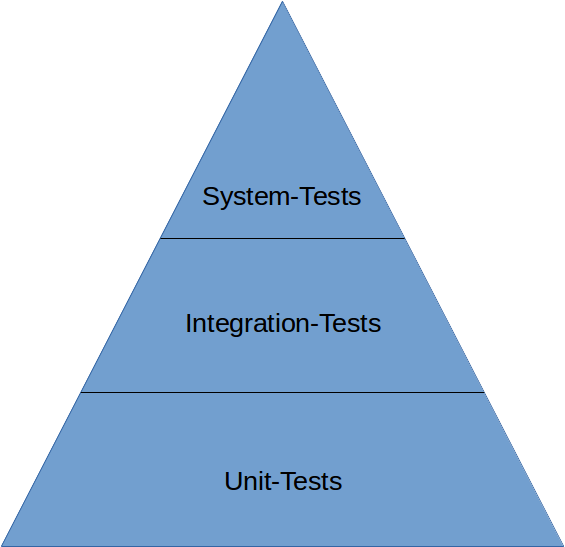
\includegraphics[scale=0.48]{img/TestPyramid.png}
\end{frame}

\begin{frame}{System test}
\begin{itemize}
  \item Test a whole (embedded) system
  \item Often automated in a Hardware-in-the-loop (HIL) system
  \item Blackbox test (internal design is unknown to the tester)
  \item Qualification test (against customer requirements)
\end{itemize}
\end{frame}

\begin{frame}{Integration test}
\begin{itemize}
  \item Test how the single modules (units) are wired
\end{itemize}
\end{frame}

\begin{frame}{Unit test}
\begin{itemize}
  \item Test the behavior of one single translation unit
\end{itemize}
\end{frame}

\subsection{Unit testing}
\begin{frame}{Unit testing}
\begin{itemize}
  \item Test only the public interface
  \item If you think a implementation detail should be tested, then it's perhaps
  an own unit
\end{itemize}
\end{frame}

\begin{frame}{A good test}
\begin{itemize}
  \item Automatic
  \item Thorough
  \item Repeatable
  \item Independent
  \item Professional
  \item Fast
\end{itemize}
\end{frame}

\subsection{Design for testability}
\begin{frame}{Design for testability}
% TODO
\end{frame}

\begin{frame}[fragile]{Unittesting in C}
Link tests, unit-under-test and test-harness to one executable
\begin{lstlisting}[language=cmake,caption=a unit test in cmake]
add_executable(TestMyModule TestMyModule.cpp MyModule.cpp)
target_link_libraries(TestMyModule gtest gtest_main)
add_test(NAME MyModule COMMAND TestMyModule)
\end{lstlisting}
\end{frame}

\subsection{Test driven development}

\begin{frame}{TDD Cycle}
\begin{enumerate}
  \item Add a test and see it fail (red)
  \item Make your test pass (green)
  \item Refactor code
\end{enumerate}
\end{frame}

\part{Version control}
\section{Version control}

\begin{frame}{Version control}
\begin{block}{What is version control}
Version control systems are a category of software tools that help a software
team manage changes to source code over time
\cite{AtlassianGitTutorials}
\end{block}
\end{frame}

\section{Git - A Distributed Version Control System}
\begin{frame}{Pro Git Book}
\url{https://git-scm.com/book}
\end{frame}

\section{Workflow}
\begin{frame}{Status}
\end{frame}

\begin{frame}{Commit}
\end{frame}

\begin{frame}{Branch}
\end{frame}

\part{Examples}

\section{Example 1}
\begin{frame}{Example 1}
\begin{itemize}
  \item Create a `Hello World` application
  \item Simple Calculator: Read two values and print sum
  \item Animal sounds: Implement classes Dog, Cat and Cow and it's base-class
  Animal, with a common makeSound() method.
\end{itemize}
\end{frame}

\section{Example 2}

\begin{frame}{Smart Pointer}
\subtitle{}
% TODO Smart Pointer example
\end{frame}

\section{Example 3}

\begin{frame}{Container}
\begin{itemize}
  \item Singly Linked List
  \item Doubly Linked List
  \item Double Ended Queue
  \item Dynamic Array
  \item Stack (LIFO)
  \item Queue (FIFO)
\end{itemize}
\end{frame}


\section{Example x}
\begin{frame}{Idioms}
http://www.programming-idioms.org/
\end{frame}

\end{document}
